\chapter{Reliable Broadcast}

\section{Links (unassessed)}
A link is a mechanism defining how two processes may interact by sending and receiving messages, and what properties hold for message passing.

\begin{definitionbox}{Fair Loss Link}
    A weak link abstraction from which other links (e.g stubborn) can be built.
    \begin{center}
        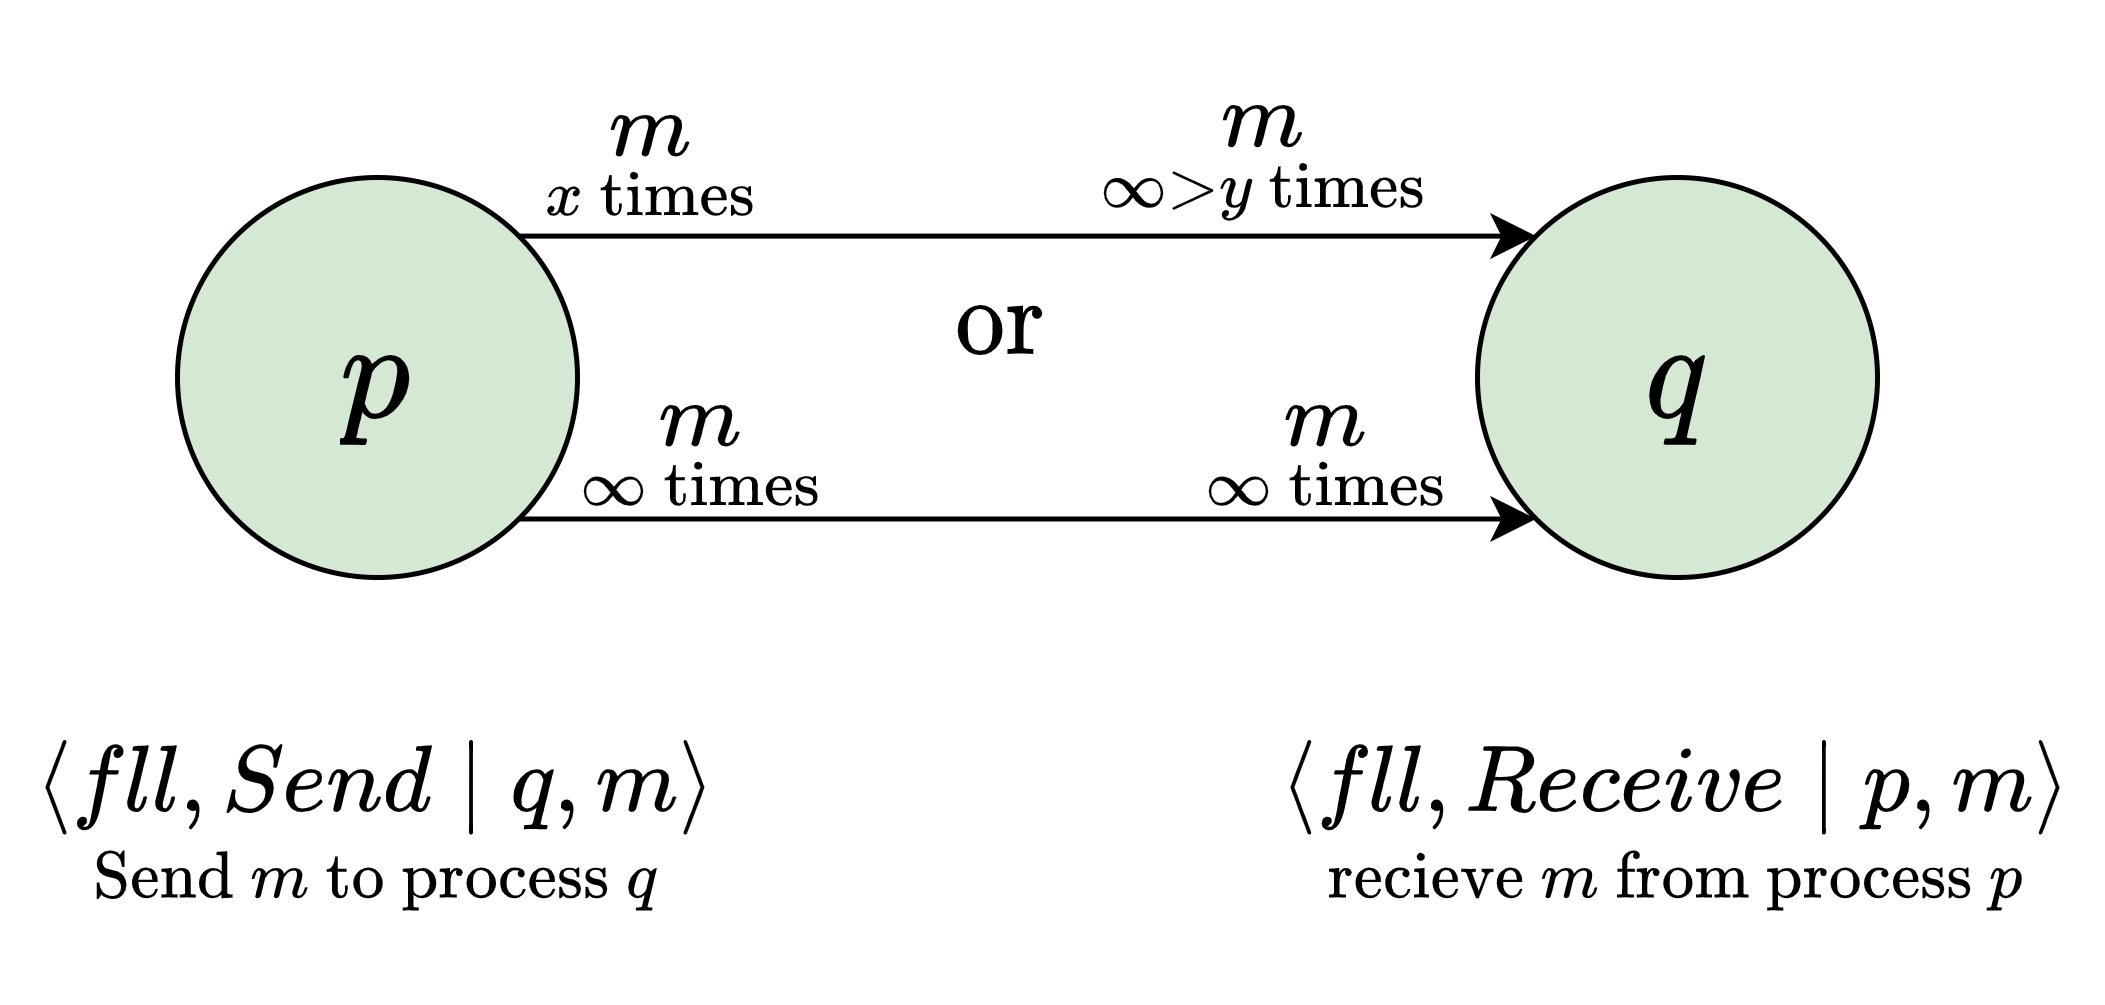
\includegraphics[width=.6\textwidth]{reliable_broadcast/images/fair_loss_links.drawio.png}
    \end{center}
    \begin{tabular}{l l p{.6\textwidth}}
        \textbf{Fair-Loss} & Liveness & Correct process $p$ infinitely sends message $m$ to correct process $q$ $\Rightarrow$ $q$ receives $m$ from $p$ infinitely many times. \\
        \textbf{Finite Duplication} & Liveness & Correct process $p$ sends message $m$ a finite number of times to $q$ $\Rightarrow$ $m$ cannot be received infinitely many times from $p$. \\
        \textbf{No Creation} & Safety & Some process $q$ receives a message $m$ with sender $p$ $\Rightarrow$ $p$ previously sent $m$ to $q$. \\
    \end{tabular}
\end{definitionbox}
\begin{definitionbox}{Stubborn Link}
    A link guaranteeing messages are received infinitely many times.
    \begin{center}
        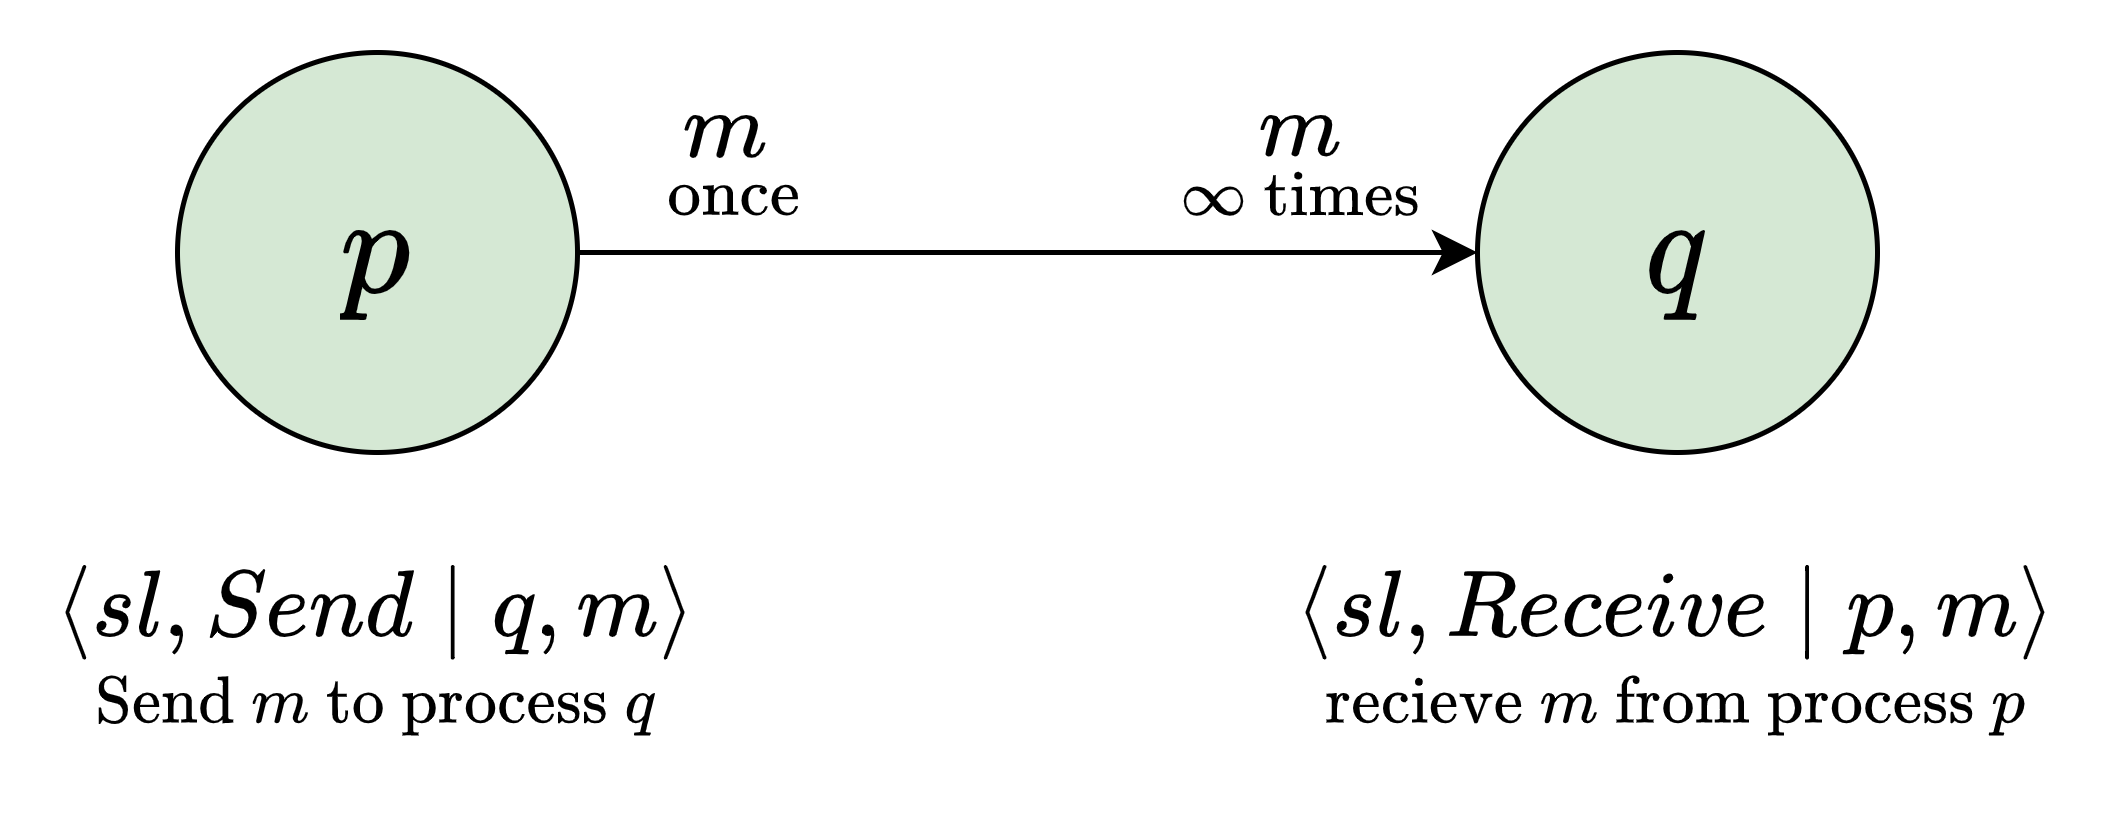
\includegraphics[width=.6\textwidth]{reliable_broadcast/images/stubborn_links.drawio.png}
    \end{center}
    \begin{center}
        \begin{tabular}{l l p{.6\textwidth}}
            \textbf{Stubborn Delivery} & Liveness & Correct process $p$ sends message $m$ to correct process $q$ $\Rightarrow$ $q$ receives $m$ from $p$ infinitely many times. \\
            \textbf{No Creation} & Safety & Some process $q$ receives a message $m$ with sender $p$ $\Rightarrow$ $p$ previously sent $m$ to $q$. \\
        \end{tabular}
    \end{center}
\end{definitionbox}

\begin{examplebox}{No change in mind}
    Implement stubborn links with elixir using the fair loss link.
    \tcblower
    
\end{examplebox}

\begin{definitionbox}{Perfect Point-to-Point Link}
    \begin{center}
        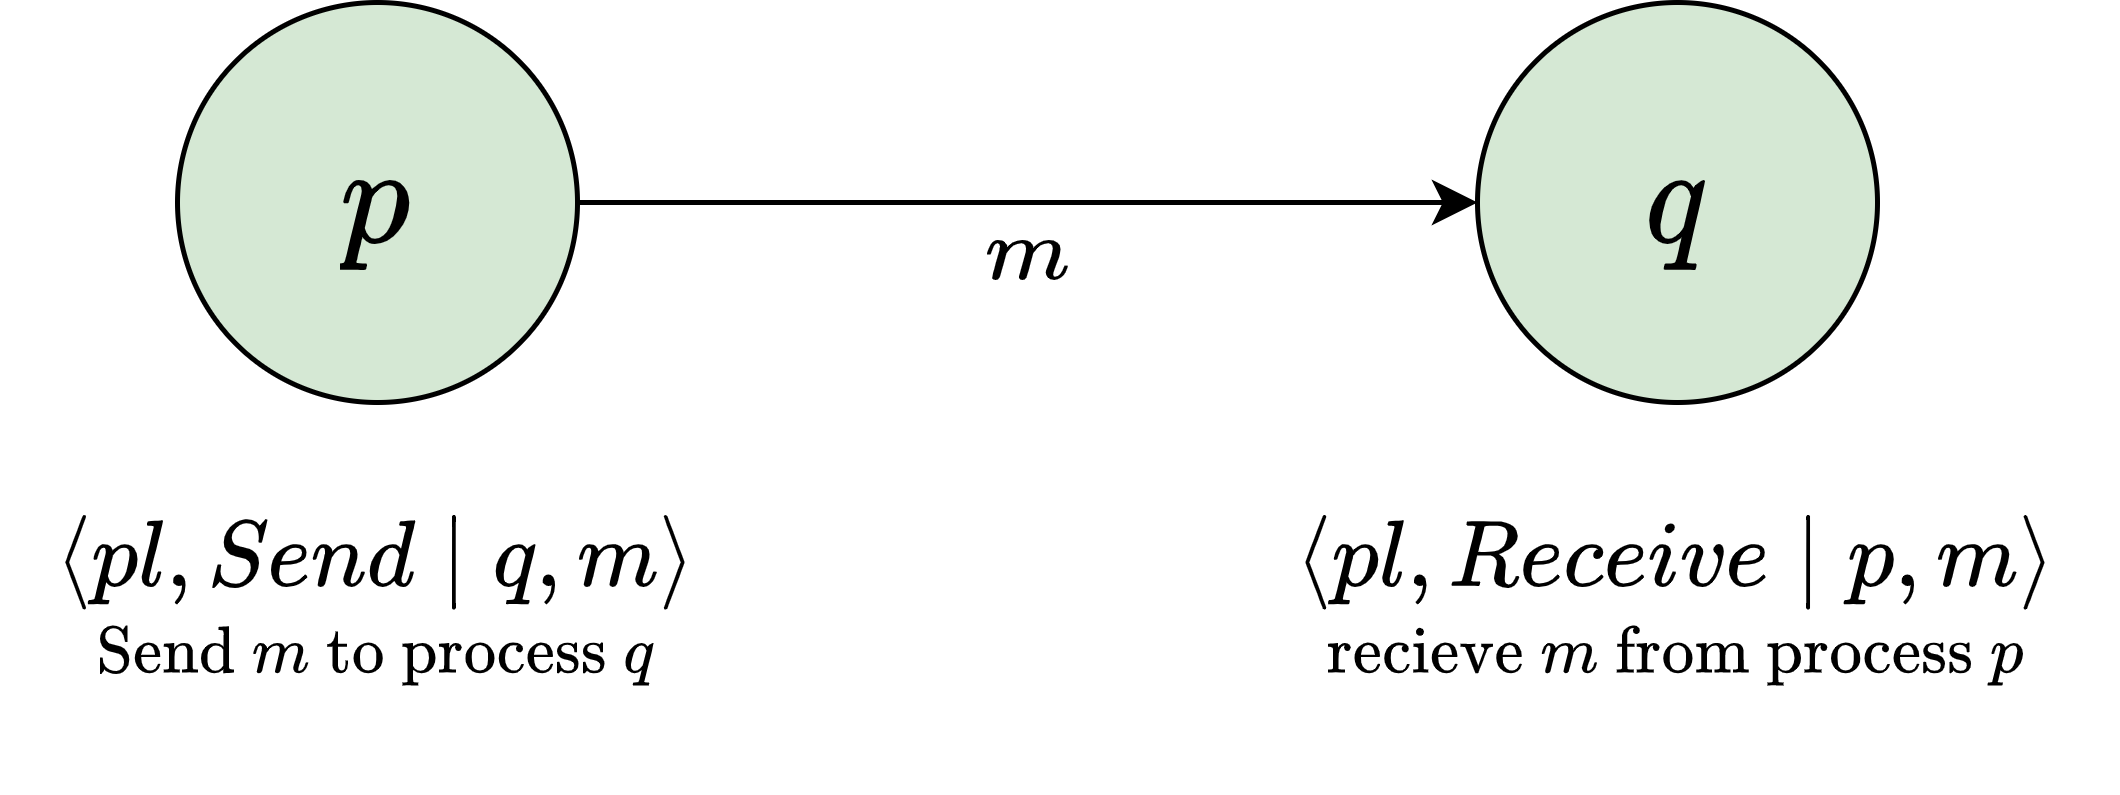
\includegraphics[width=.6\textwidth]{reliable_broadcast/images/perfect_links.drawio.png}
    \end{center}
    \begin{itemize}
        \item Also called \textit{reliable message passing}
    \end{itemize}
    \begin{center}
        \begin{tabular}{l l p{.6\textwidth}}
            \textbf{Reliable Delivery} & Liveness & Correct process $p$ sends $m$ to correct process $q$ $\Rightarrow$ $q$ will eventually receive $m$. \\
            \textbf{No Duplication} & Safety & No message is received by a process more than once. \\
            \textbf{No Creation} & Safety & Some process $q$ receives a message $m$ with sender $p$ $\Rightarrow$ $p$ previously sent $m$ to $q$. \\
        \end{tabular}
    \end{center}
\end{definitionbox}

\section{Failure Detection}
A failure detector provides a process with a list of \textit{suspected processes}.
\begin{itemize}
  \item Failure detectors make, and encapsulate some timing assumptions in order to determine which processes are suspect.
  \item They are not fully accurate, and their specification allows for this.
\end{itemize}

\begin{definitionbox}{Perfect Failure Detector}
  A failure detector that is never incorrect / is entirely accurate.
  \begin{itemize}
    \item Never changes its view on failure $\to$ once detected as crashed it cannot be \textit{unsuspected}.
    \item Often represented as $\mathcal{P}$
  \end{itemize}
  \begin{center}
    \begin{tabular}{l l p{.6\textwidth}}
      \textbf{Strong Completeness} & Liveness & Eventually every process that crashes is permanently detected as crashed by every correct process. \\
      \textbf{Strong Accuracy} & Safety & $p$ detected $\Rightarrow$ $p$ has crashed. \\
    \end{tabular}
\end{center}
\end{definitionbox}

\begin{definitionbox}{Eventually Perfect Failure Detector}
  A failure detector that is not entirely accurate.
  \begin{itemize}
    \item Can restore processes (no longer suspected).
    \item Often represented as $ \lozenge  \mathcal{P}$
  \end{itemize}
  \begin{center}
    \begin{tabular}{l l p{.6\textwidth}}
      \textbf{Strong Completeness} & Liveness & Eventually every process that crashes is permanently detected as crashed by every correct process.  \\
      \textbf{Eventual Strong Accuracy} & Liveness & Eventually no correct process is suspected by any other correct process \\
    \end{tabular}
\end{center}
\end{definitionbox}

\section{One-Shot Communication}


\subsection{Best Effort Broadcast}
\begin{definitionbox}{Best Effort Broadcast}
    A non-reliable, single-shot broadcast.
    \begin{itemize}
        \item Only reliable if the broadcasting process is correct during broadcast (if crashing during broadcast only some messages may be delivered, and processes may disagree on delivery)
        \item No delivery agreement guarantee (correct processes may disagree on delivery)
        \item Uses \textit{Perfect Point-to-Point Link} and inherits properties from it.
    \end{itemize} 
    \begin{center}
        \begin{tabular}{l l p{.6\textwidth}}
            \textbf{Validity} & Liveness & If a correct process broadcasts a message then every correct process eventually receives it. \\
            \textbf{No Duplication} & Safety & No message is received by a process more than once. \\
            \textbf{No Creation} & Safety & No broadcast is delivered unless it was broadcast. \\
        \end{tabular}
    \end{center}
\end{definitionbox}
We can implement this in elixir using the send and receive primitives as \textit{Perfect Point-to-Point Link}.
\begin{minted}{elixir}
# Broadcast using perfect point-to-point links
# processes <- the list of processes in the broadcast space
# pl        <- the perfect links process to use
# c         <- the object broadcasting & being delivered
defmodule Best_Effort_Broadcast do
  def start(processes) do
    receive do {:bind, pl, c} -> next(processes, pl, c)
  end

  defp next(processes, pl, c) do
    receive do
      {:beb_broadcast, msg} -> 
        for dest <- processes do
            send pl, {:pl_send, dest, msg}
        end
      {:pl_deliver, src, msg} ->
        send c, {:beb_deliver, src, msg}
    end
    next (processes, pl, c)
  end
end
\end{minted}


\subsection{Reliable Broadcast}
\begin{definitionbox}{Reliable Broadcast}
    Adds a delivery guarantee to \textit{best effort broadcast}  
    \begin{center}
        \begin{tabular}{l l p{.6\textwidth}}
            \textbf{Agreement} & Liveness & If a correct process delivers message $m$ then all correct processes deliver $m$ \\
            \multicolumn{3}{c}{\textbf{All Properties from Best Effort Broadcast}} \\
        \end{tabular}
    \end{center}
    The combination of \textbf{Validity} and \textbf{Agreement} form a \textit{termination property} (system reaches agreement in finite time).
\end{definitionbox}
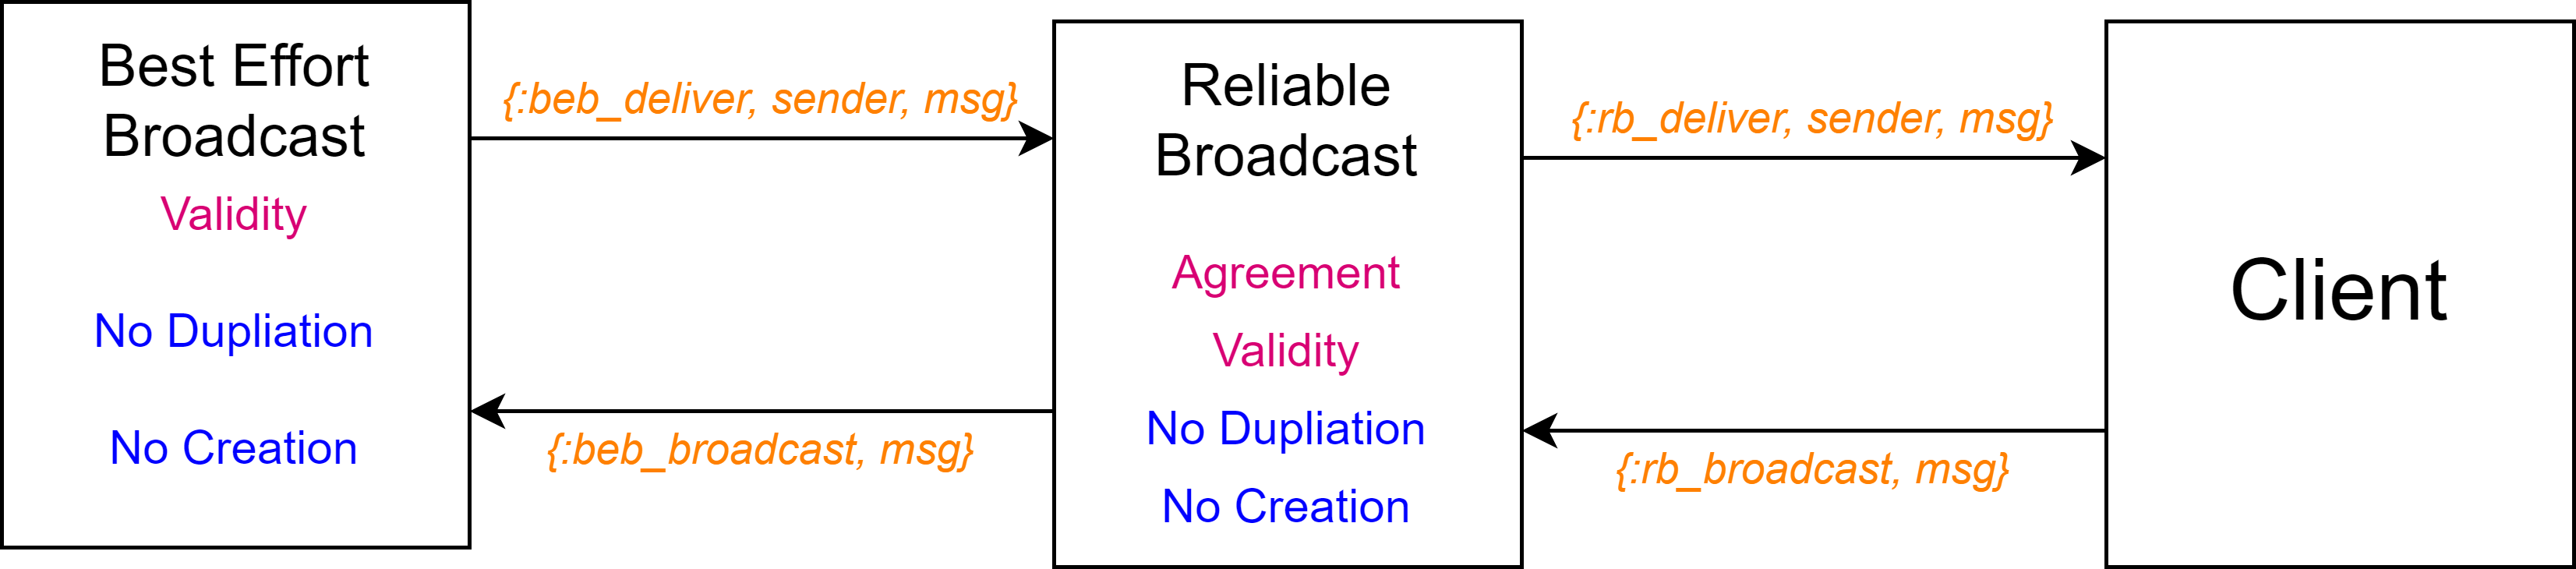
\includegraphics[width=.8\textwidth]{reliable_broadcast/images/reliable_broadcast.drawio.png}

\subsection{Eagre Reliable Broadcast}
\begin{definitionbox}{Eagre Reliable Broadcast}
    A \textit{reliable broadcast} where every process re-broadcasts every message it delivers.
    \begin{itemize}
        \item If the broadcasting process crashes, and only some correct processes deliver the message, then re-broadcast ensures eventually all will receive.
        \item This broadcast is \textit{fail-silent}
        \item Very inefficient to implement, broadcast to $n$ processes results in $O(n^2)$ messages.
        \item \textbf{Validity} property combined with retransmission provides \textbf{agreement}.
    \end{itemize}
    \begin{center}
        \begin{tabular}{l l p{.6\textwidth}}
            \multicolumn{3}{c}{\textbf{All Properties from Reliable Broadcast}} \\
        \end{tabular}
    \end{center}
\end{definitionbox}

\begin{minted}{elixir}
# Eagre reliable broadcast implemented using Best Effort Broadcast
# beb <- the best effort broadcast process
# c   <- the object broadcasting & being delivered
defmodule Eagre_Reliable_Broadcast do

  def start do
    receive do { :bind, c, beb } -> next(c, beb, MapSet.new) end
  end

  defp next(c, beb, delivered) do
    receive do
      { :rb_broadcast, msg } ->
        send beb, { :beb_broadcast, { :rb_data, our_id(), msg } }
        next(c, beb, delivered)
      { :beb_deliver, from, { :rb_data, sender, msg } = rb_m } ->
        if msg in delivered do
          # Message was already delivered, so can be ignored
          next(c, beb, delivered)
        else
          # Message is new, so add to delivered, deliver to c & rebroadcast
          send c, { :rb_deliver, sender, msg }
          send beb, { :beb_broadcast, rb_m }
          next(c, beb, MapSet.put(delivered, msg))
        end
    end
  end

end
\end{minted}

\subsubsection{Lazy Reliable Broadcast}
\begin{definitionbox}{Lazy Reliable Broadcast}
    A \textit{reliable broadcast} using \textit{Best Effort Broadcast} with a \textit{Failure Detector} to enforce agreement.
    \begin{itemize}
        \item Uses a \textit{perfect failure detector}.
        \item When a process is detected to have crashed, all broadcasts delivered from the process are rebroadcasted
        \item Agreement is derived from the \textbf{validity} of \textit{best effort broadcast}, that every correct process broadcasts every message delivered from a crashed process and the properties of the \textit{perfect failure detector}.
    \end{itemize}
\end{definitionbox}

\begin{center}
  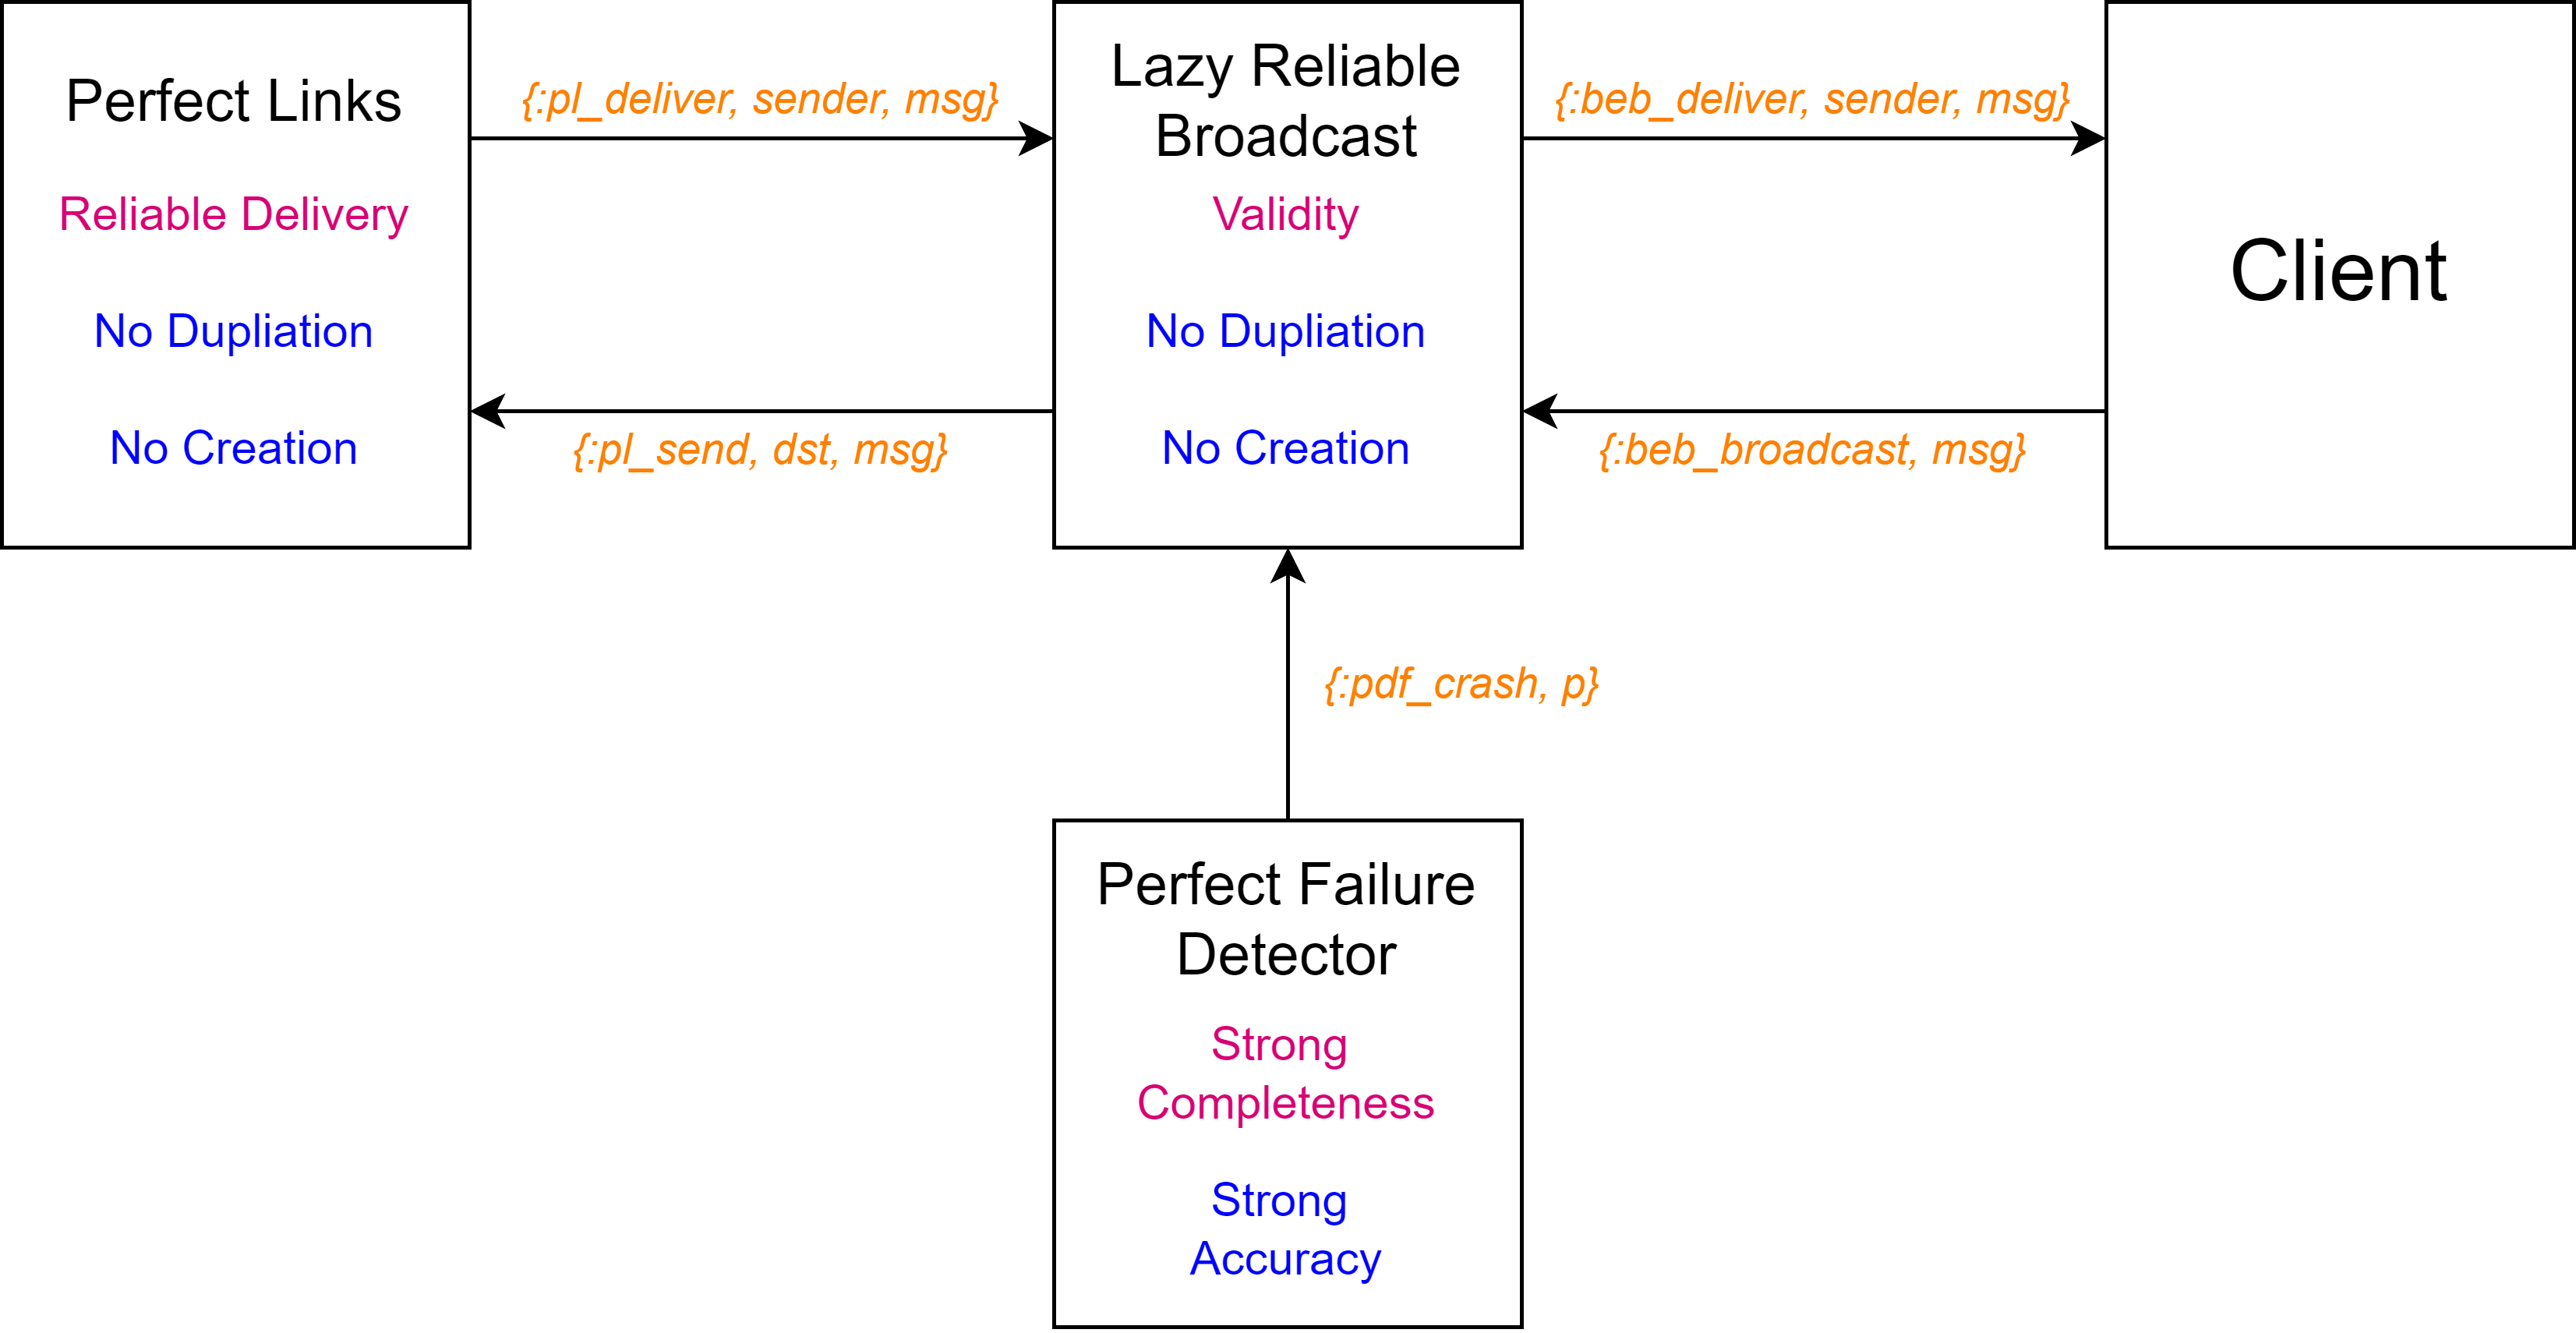
\includegraphics[width=.8\textwidth]{reliable_broadcast/images/lazy_reliable_broadcast.drawio.png}
\end{center}

\begin{minted}{elixir}
# Lazy Reliable Broadcast implemented using best effort broadcast
# beb    <- the best effort broadcast process
# client <- the object broadcasting & being delivered
defmodule Lazy_Reliable_Broadcast do
  def start do
    receive do
      { :bind, processes, client, beb } ->
        delivered = Map.new(processes, fn p -> {p, MapSet.new} end)
        next(client, beb, processes, delivered)
    end
  end

  defp next(client, beb, correct, delivered) do
    receive do
      { :rb_broadcast, msg } ->
        # broadcast a message with our id
        send beb, { :beb_broadcast, { :rb_data, our_id(), msg } }
        next(client, beb, correct, delivered)

      { :pfd_crash, crashedP } ->
        # Failure detector has detected a crashed process
        # For each message delivered by the crashed process,
        # rebroadcast (from them)
        for msg <- delivered[crashedP] do
          send beb, { :beb_broadcast, { :rb_data, CrashedP, msg } }
        end
        next(c, beb, MapSet.delete(correct, crashedP), delivered) # cont

      { :beb_deliver, from, { :rb_data, sender, msg } = rb_m } ->
        # A message is delivered, if already received do nothing,
        # otherwise record the delivered message,
        if msg in delivered[sender] do
          next(c, beb, correct, delivered)
        else
          send c, { :rb_deliver, sender, msg }
          # add msg to the set of messages received from sender
          sender_msgs = MapSet.put(delivered[sender], msg)
          delivered = Map.put(delivered, sender, sender_msgs)

          # The sender may have since crashed, so may need to
          # rebroadcast
          if sender not in correct do
            send beb, { :beb_broadcast, rb_m }
          end

          next(c, beb, correct, delivered)
      end
    end
  end

end
\end{minted}

\subsection{Uniform Reliable Broadcast}



\section{Multi-Shot Communication}

